\documentclass{article}
\usepackage{graphicx} % Required for inserting images
% \usepackage{oxycomps}

\title{Junior Seminar - GitHub Tutorial}
\author{Zahir Choudhry}
\date{February 10th, 2024}
\begin{document}
\maketitle
\hrule

\vspace{15pt}
% Introduction Paragraph
\centering The goal of this paper is to teach people about what Github is and how to utilize it, as well as issues you may face when using it.
This tutorial will be utilizing Bash commands in Terminal (Mac), but there are alternaticve ways to use Github such as Gitkraken and Github Desktop.

\vspace{15pt}

% Table of Contents
\section*{\underline{Table of Contents}}
\subsection*{{Basic Concepts:}}

\begin{itemize}
\item Init-ing / Cloning
\item Adding
\item Commiting
\item Pushing

\subsection*{\centering{Advanced Concepts:}}
\item Plus Stashes
\item Branches
\item Merging
\item Dealing with Conflicts
\end{itemize}

\vspace{50pt}   

\vspace{20pt}
% 4 Stages of Github
\section*{4 Data Stores of Github}

\vspace{15pt}
% 4 Stages Picture
\begin{figure}[h]
    \centering
    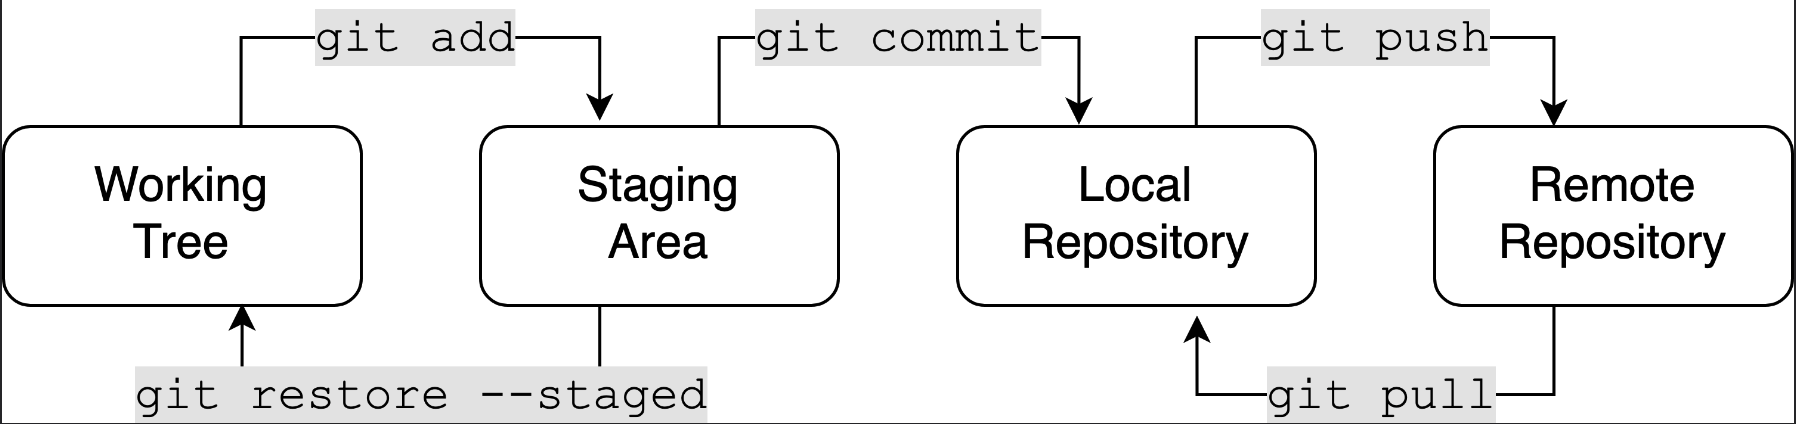
\includegraphics[width=0.9\textwidth]{Map.png}
    \caption{ The 4 Data Stores of Git}
    \label{fig:example}
\end{figure}

\vspace{15pt}
\hrule

% Explanations:
\subsection*{Working Tree}
The Working Tree is where the user makes changes to their files. It is the project directory on a user's local device. Basically, it is the files on a user's computer.
\vspace{15pt}

\subsection*{Staging Area}
The Staging Area is the intermediate area where a file goes before it is committed to Github. Allows the user to check their changes and make sure there will be no conflict with other files that are also staged or going to be committed.
\vspace{15pt}

\subsection*{Local Repository}
The Local Repository is a copy or clone of a user's Github Repository that resides on their computer. The Local Repository will contain the history of your Github project, including all branches, commits and version control information. Allows for users to work on their projects offline and collaborate with others.
\vspace{15pt}

\subsection*{Remote Repository}
The Remote Repository is a repository hosted on another server from your own device. It serves as the version of your project that others can clone and work on, and is where you want to commit your most recent version of your code.
\vspace{5pt}

\section*{Basic Concepts}
\hrule
\vspace{25pt}
\subsection*{Init-ing / Cloning}
Init-ing and Cloning are 2 commands that create new Github repositories on your local directory. However, there is a crucial difference between the two commands. Init-ing create a completely brand new blank repository in you directory, while git clone will pull a copy of an existing repository from a remote server onto your local device.
\vspace{15pt}
\subsection*{Adding}
Adding is putting a file into the Staging Area. This area is still on your local device and is one level below committing your work. You must add a work before committing it. Adding is important because it allows developers to see what they may be committing that they may not want to, like conflicts or SSHs/Keys that they intended to delete.
\vspace{15pt}
\subsection*{Committing}
Committing is the second step, moving from the Staging Area into the Local Repository. Once a file is committed, it is saved in the version control history, which is why the Staging Area is important, allowing users to look over their code one last time before it is permanently saved into Git's history. When a user makes a commit, a message editor pops up asking for a 'commit message'. This message allows users to provide detailed information on the changes they've made, making it easier for others trying to work on the code to understand how they can help and what has already been accomplished.
\vspace{15pt}
\subsection*{Pushing}
Finally, Pushing is moving the files from the Local Repository to the Remote Repository. Your project files are finally off your computer and on a separate server that other users can use to clone your project and work on it. It is a good practice to check that your Local Repository and Remote Repository are synced up using 'git fetch' or 'git pull'. When first pushing to a Remote Repository, the user has to specify both which Remote Repository and which Branch they intend to push to. When pushing to private server, users will be prompted with an authentication screen. 
\vspace{55pt}

\section*{Advanced Concepts}
\hrule
\vspace{15pt}

\subsection*{Stashes}
Stashing is a technique that allows users to temporarily not add certain changes in your Working Tree so that users can work on another task, and then come back and apply those changes when they are ready. Users can choose to apply changes from their stashes or delete them instead.

\subsection*{Branches}
\begin{figure}[h]
    \centering
    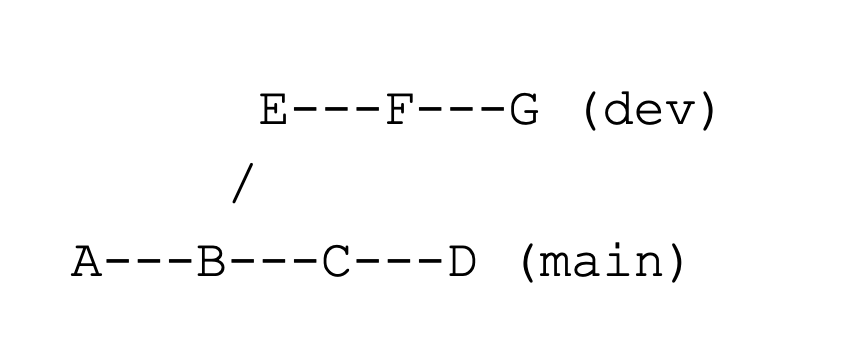
\includegraphics[width=0.5\textwidth]{branch.png}
\end{figure}
A Branch is like when a specific commit has 'multiple children'. Branches allow users to have parallel development, with one branch being used to work on one feature and another work on a different one for the same project, allowing for the two ideas to fully fleshed out before being combined into a final product.
\subsection*{Merging}
\begin{figure}[h]
    \centering
    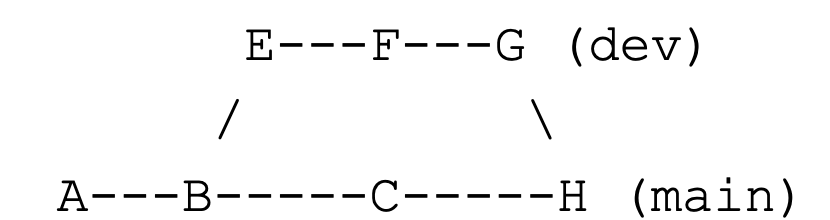
\includegraphics[width=0.5\textwidth]{Merge.png}
\end{figure}
Merging is when 2 branches are combined back together into one branch. While it seems simple, there are many opportunities for conflicts when merging. A conflict occurs when both files try to overwrite the same things, leaving the computer confused on what is the correct one to follow. When a conflict occurs, the merge is halted and marks files with conflicting information. The merge will resume once the user deals with the conflicts and re-instates the merge. 
\vspace{45pt}

\section*{Examples of Conflicts}
\hrule
\vspace{15pt}
\begin{itemize}
    \item Same line in both branches have different modifications
    \item File deleted in one branch, modified in another
    \item Directory names not the same
    \item Whitespace and Formatting
    \item Binary Files (Images/Compiled Binaries): Github can't perform a line-by-line merge on binary files. If both branches modify a binary file, Git marks it as a conflict 
\end{itemize}

\end{document}
